\documentclass[12pt]{article}
\usepackage[utf8]{inputenc}
\usepackage{hyperref}
\usepackage{graphicx}

\title{Era of Compute Specialization}
\author{Shaan Fulton}
\date{\today}

\begin{document}

\maketitle

\section*{Moore's Law}

Gordon Moore's prediction that transistor count on an integrated circuit is expected to double roughly every two years. This has roughly continued since 1970. Notably, this says nothing about performance.

\begin{figure}[h]
    \centering
    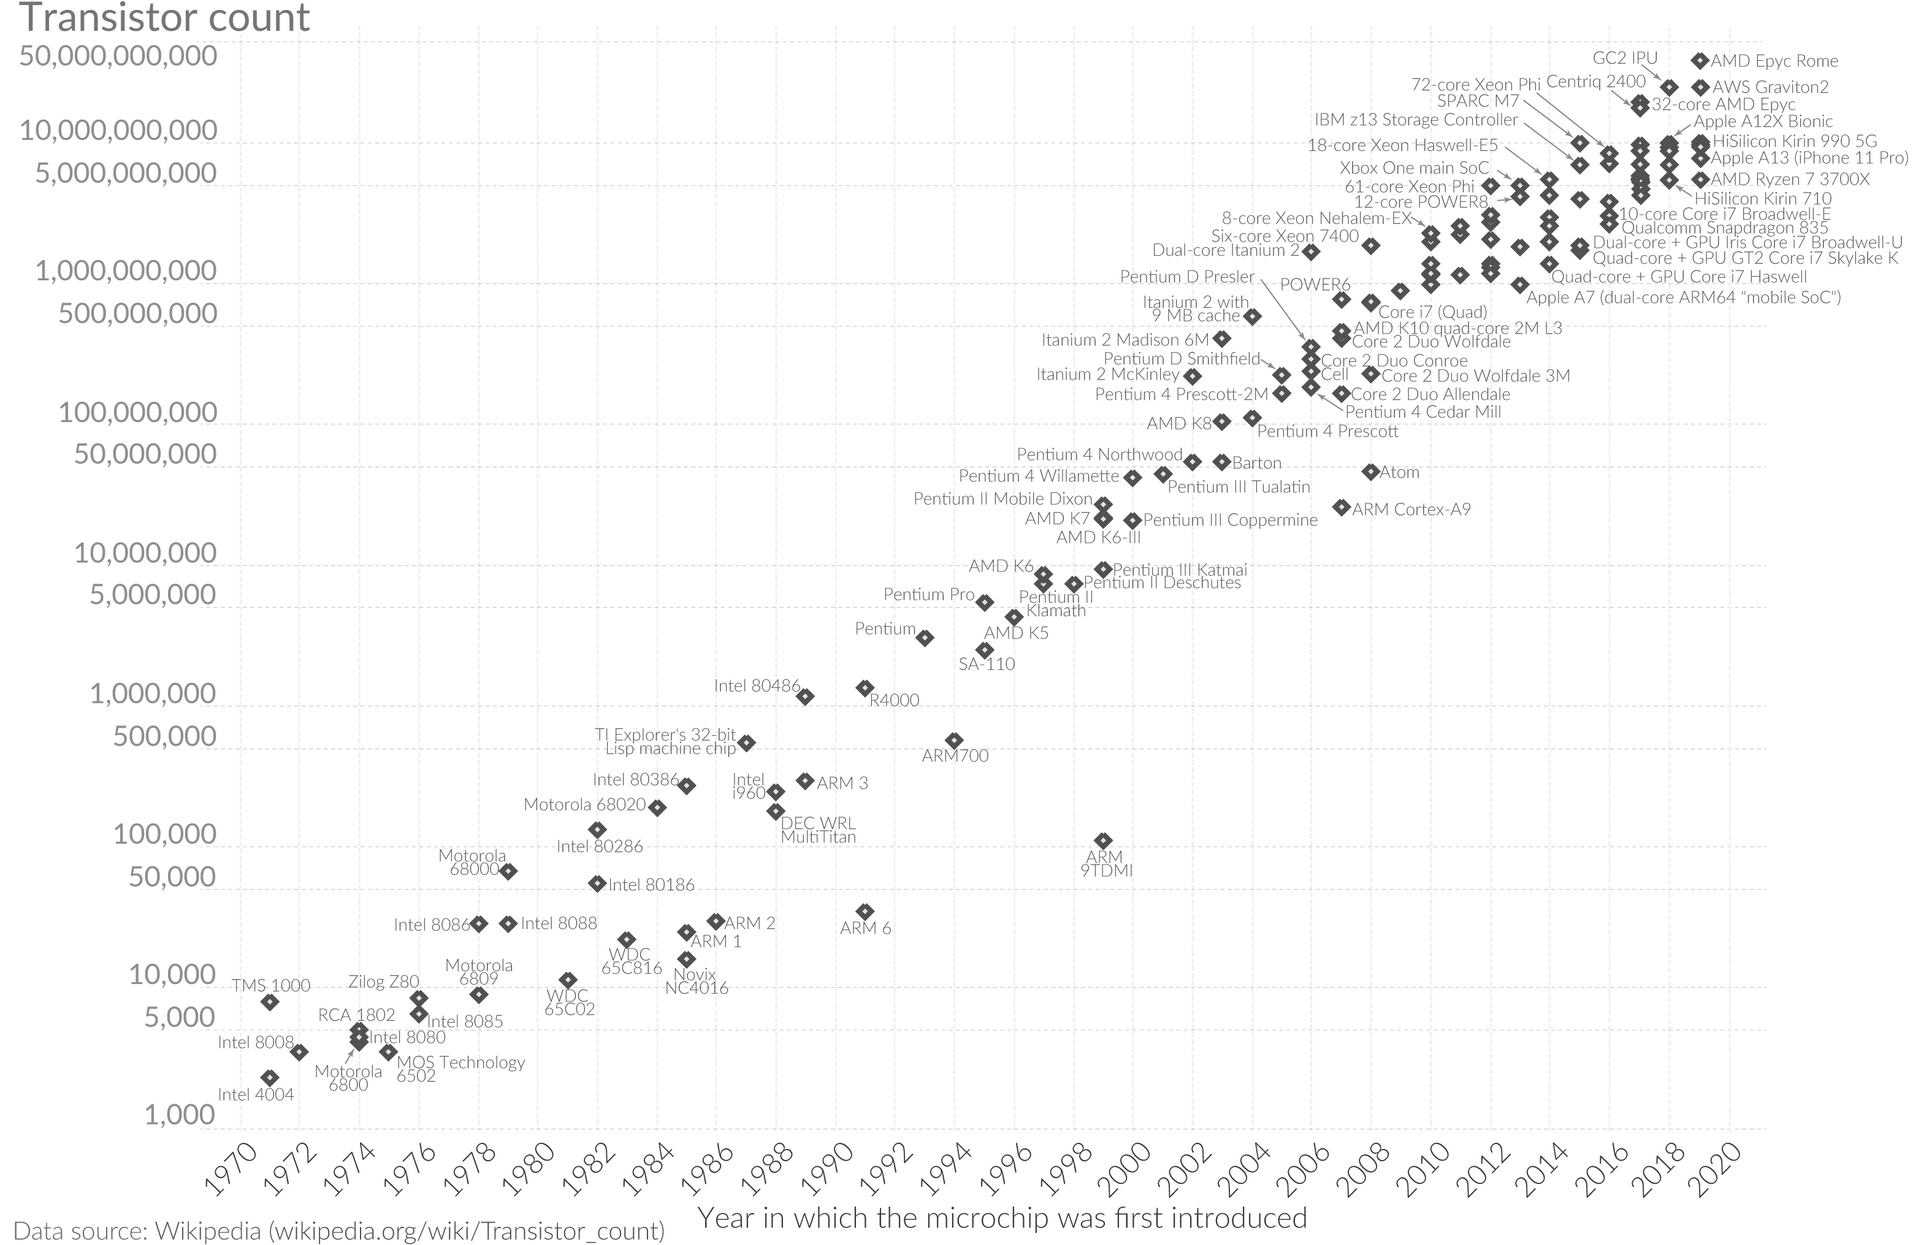
\includegraphics[width=1\textwidth]{moores.png}
    \caption{Transistor count over time.}
\end{figure}

\section*{Amdahl's Law}

When a metric of performance is considered, the picture changes drastically. No matter how many cores you add, if your processes are serialized, the number of active cores at once is significantly diminished. You have a board full of useless transistors. \textbf{Ambdahl's Law} states that every process is ultimately bottlenecked by the necessarily serial components of it. No matter how beautifully you parallelize half of your program, the bottleneck will remain in the other half which must be serialized. Still, through effective algorithm and software design we can parallelize numerical processes and continue to see performance gains.

\begin{figure}[h]
    \centering
    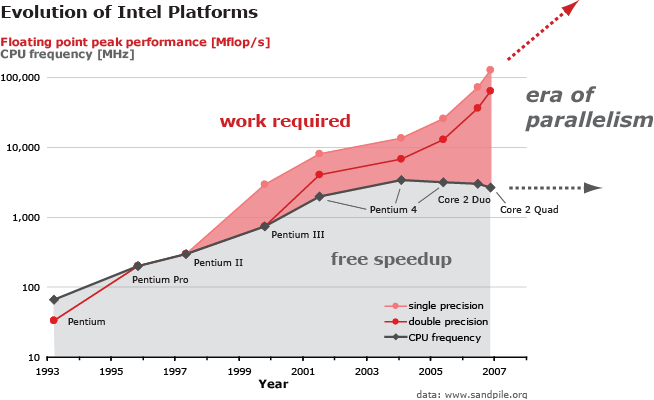
\includegraphics[width=1\textwidth]{amdahls.png}
    \caption{Transistor count over time.}
\end{figure}

\section*{Compute Specialization}

We see from Amdahl's Law that software can only be optimized so much. The new paradigm in computing, therefore, is designing specialized chipset for specific operations. This becomes extremely apparent as soon as you consider the modern computing landscape: The advent of the GPU and TPU are recent and compelling examples. Arguably, the future of computing is in these specialized compute units. We can no longer rely on the general purpose processer to push computing forward.

\end{document}

